\chapter{Simulation}
\section{Geometric Simulation}

A kinematic workspace is a visual representation of possible end effector positions in a specific coordinate system. In the case of Baleka, a polar coordinate system was used with the foot of the robot being the end effector. The leg model with relevant coordinates can be seen in \cref{fig:Geometric view of leg} and will be referred to further in the discussion below.

The kinematic workspace generated by various linkage length combinations was compared in order to properly choose an appropriate configuration. 

In order to perform a geometric simulation of all possible foot positions Matlab was used, the code in mention can be seen in \cref{listing:Geometric simulation code}. 

A grid of all $\phi_1$ and $\phi_2$ motor angles was generated. It was assumed that the angles would be limited to a range of between $20^o$ and $180^o$ from vertical. Using the forward kinematic equation from \cref{chap:kinematics} all possible $r$ and $\theta$ pairs were generated and subsequently plotted to produce the kinematic workspaces in \cref{fig:Polar co-ordinates generated 5-30,fig:Polar co-ordinates generated 15-30,fig:Polar co-ordinates generated 30-30,fig:Polar co-ordinates generated 30-15}.

\subsection{Data Analysis}
The plots were generated with a motor angle resolution of $0.125\ radians$. In reality the motor encoders used had a 500 count resolution and could therefore accurately measure at $0.0125\ radian$ steps. For better visual representation the lower resolution was used. 

It can be clearly seen that at the extremes of the radial range the points plotted are more dense. This indicates that a higher resolution movement can be achieved at these points. This is expected due to the more acute joint angles when at these positions. Realistically for a system with mechanical slack this has little useful effect, but theoretically the higher resolution at extended foot positions would be of use for fine tuned launch and landing control were the leg would either be extended or compressed. 

There are three points of interest on the kinematic workspace plots:
\begin{enumerate}
\item Radial position of greatest angular movement.
\item Minimum achievable radius.
\item Maximum achievable radius.
\end{enumerate}

\subsubsection{$l_1=5\ cm$ and $l_2=30\ cm$}
For leg linkage lengths of $l_1=5\ cm$ and $l_2=30\ cm$ in \cref{fig:Polar co-ordinates generated 5-30} the radial position of greatest angular movement is $r=0.3\ m$. The radius varies from $0.35\ m$ at its greatest down to $0.25\ m$. 

The position of greatest angular movement is ideally positioned in the middle of the radial range providing a well spaced workspace. 

The radial range of only $10\ cm$ is limiting and not ideal for jumping which requires maximum radial range to ensure the foot is in contact with the ground for as long possible when launching.

\subsubsection{$l_1=15\ cm$ and $l_2=30\ cm$}
For leg linkage lengths of $l_1=5\ cm$ and $l_2=30\ cm$ in \cref{fig:Polar co-ordinates generated 15-30} the radial position of greatest angular movement is just above $r=0.3\ m$. The radius varies from $0.45\ m$ at its greatest down to $0.15\ m$. 

The position of greatest angular movement is ideally positioned in the middle of the radial range providing a well spaced workspace. 

The radial range of $30\ cm$ is adequate for single leg hopping, but would maybe need to be increased for full body robotic movement.

\subsubsection{$l_1=30\ cm$ and $l_2=30\ cm$}
For leg linkage lengths of $l_1=30\ cm$ and $l_2=30\ cm$ in \cref{fig:Polar co-ordinates generated 30-30} the radial position of greatest angular movement is near to zero. The radius varies from $0.6\ m$ at its greatest down to $0\ m$. 

The position of greatest angular movement is positioned at near zero which is of little benefit to robotic hopping movement where maximum angular movement is needed when the leg is extended.

The radial range of $60\ cm$ is large, but with the drawbacks mentioned above.

\subsubsection{$l_1>l_2$}
As soon as $l_2$ is greater than $l_2$ the forward kinematic mapping from \cref{chap:kinematics} produces imaginary values of radius. This can be seen in \cref{fig:Polar co-ordinates generated 30-15} where complex values were not plotted leaving gaps in the kinematic workspace. 

In practise it is difficult to properly implement complex calculations on an embedded system and it is better avoided all together. 

\subsubsection{Conclusion}
The simulation of $l_1=15\ cm$ and $l_2=30\ cm$ provided the best combination of maximum radial length and range while placing the radial position of greatest angular movement midway between the two extreme limits. 

A linkage ratio of $\frac{1}{2}$ should be used, with linkage length being decided upon based on motor current requirements where a longer leg produces more torque at the extreme foot positions and will therefore use a higher current. 

The motor current simulation with a linkage length of $l_1=15\ cm$ and $l_2=30\ cm$ was performed in \cref{fig:motor-current-requirements} - this combination of linkage lengths was found to be ideal for the BLDC motors and motor drivers available.

\begin{figure}
\centering
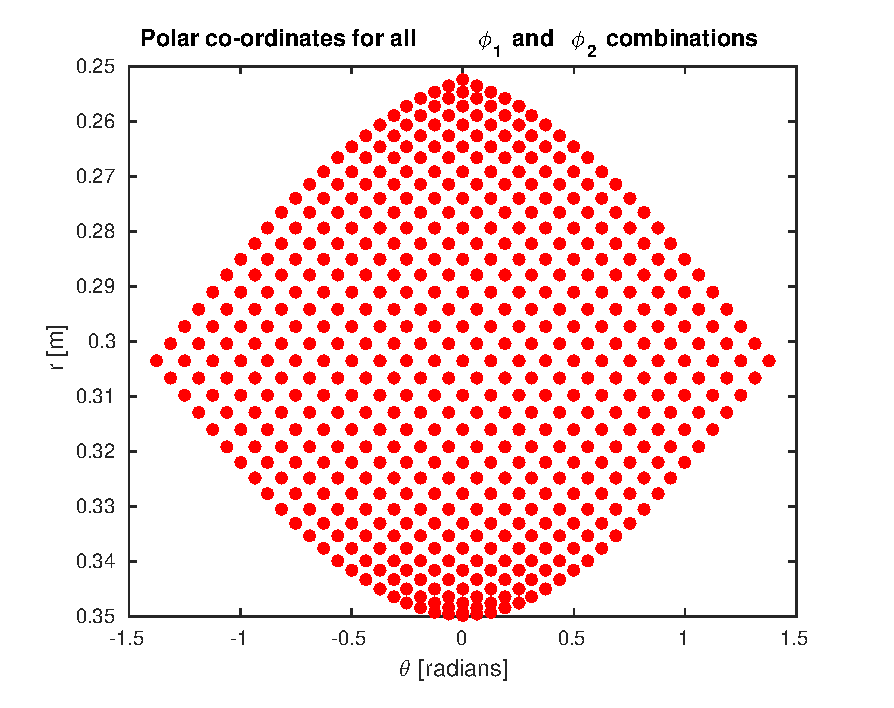
\includegraphics[width=0.8\textwidth]{images/geometry/forward-kinematic-leg-positions-5-30.eps}
\caption{Polar co-ordinates generated for all $\phi_1$ and $\phi_2$ combinations using forward kinematics: $l_1 = 5cm\ l_2 = 30cm$.}
\label{fig:Polar co-ordinates generated 5-30}
\end{figure}

\begin{figure}
\centering
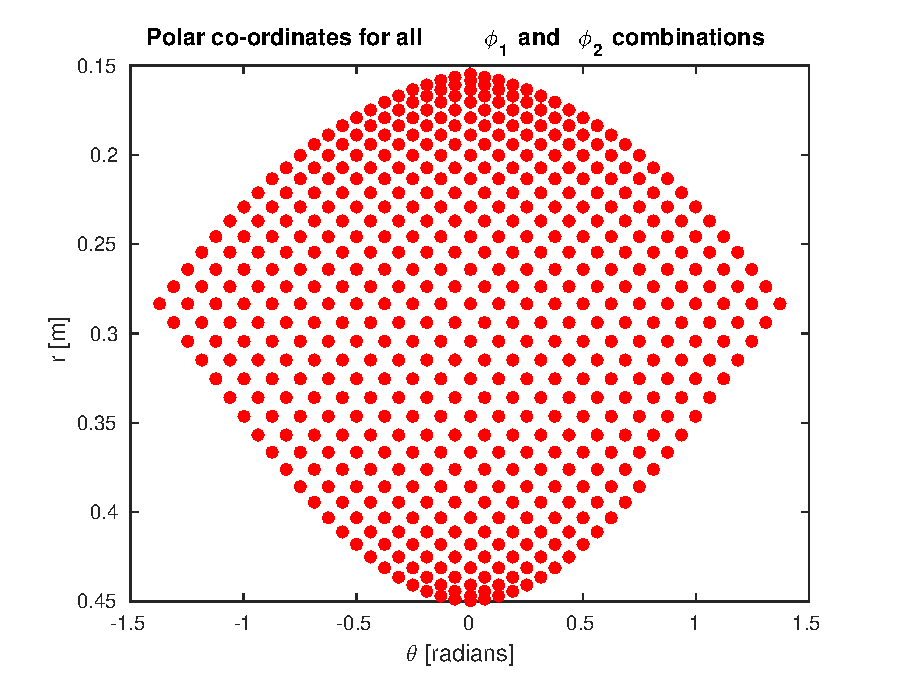
\includegraphics[width=0.8\textwidth]{images/geometry/forward-kinematic-leg-positions.eps}
\caption{Polar co-ordinates generated for all $\phi_1$ and $\phi_2$ combinations using forward kinematics: $l_1 = 15cm\ l_2 = 30cm$.}
\label{fig:Polar co-ordinates generated 15-30}
\end{figure}

\begin{figure}
\centering
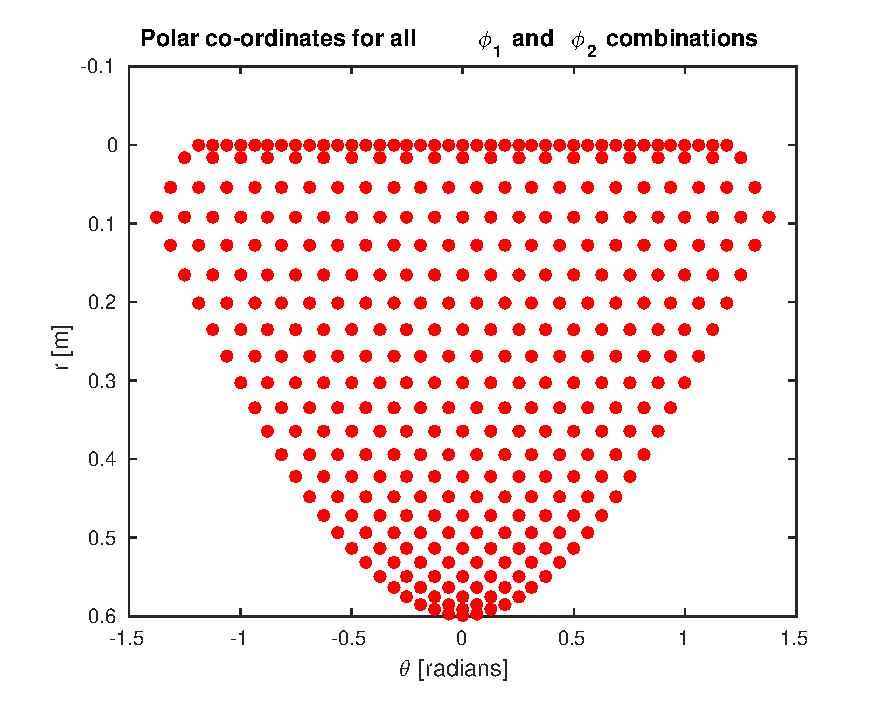
\includegraphics[width=0.8\textwidth]{images/geometry/forward-kinematic-leg-positions-30-30.eps}
\caption{Polar co-ordinates generated for all $\phi_1$ and $\phi_2$ combinations using forward kinematics: $l_1 = 30cm\ l_2 = 30cm$.}
\label{fig:Polar co-ordinates generated 30-30}
\end{figure}

\begin{figure}
\centering
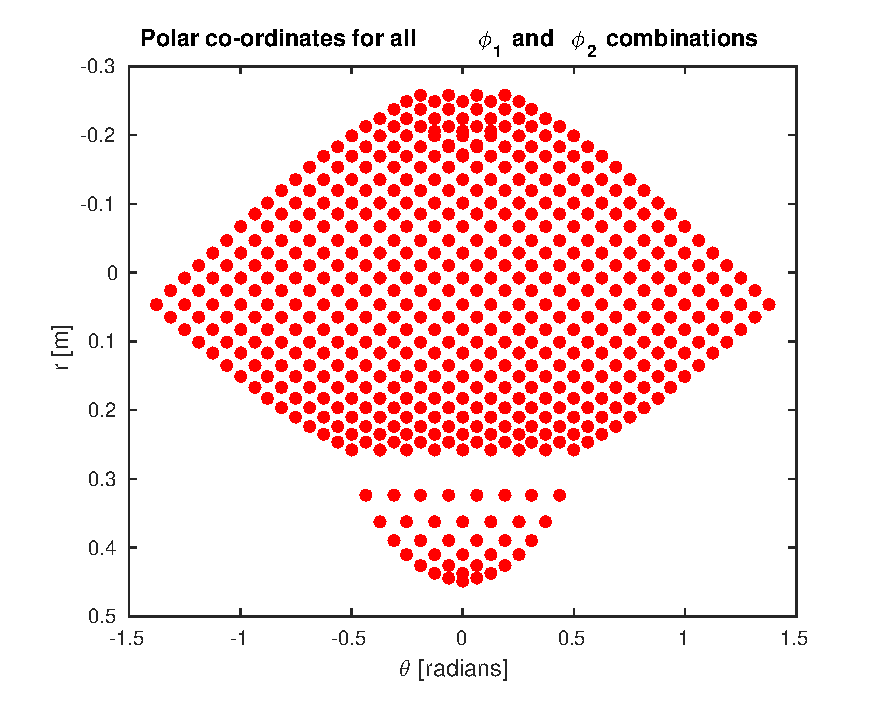
\includegraphics[width=0.8\textwidth]{images/geometry/forward-kinematic-leg-positions-30-15-complex.eps}
\caption{Polar co-ordinates generated for all $\phi_1$ and $\phi_2$ combinations using forward kinematics: $l_1 = 30cm\ l_2 = 15cm$.}
\label{fig:Polar co-ordinates generated 30-15}
\end{figure}

\section{Control Simulation}

\begin{figure}
\centering
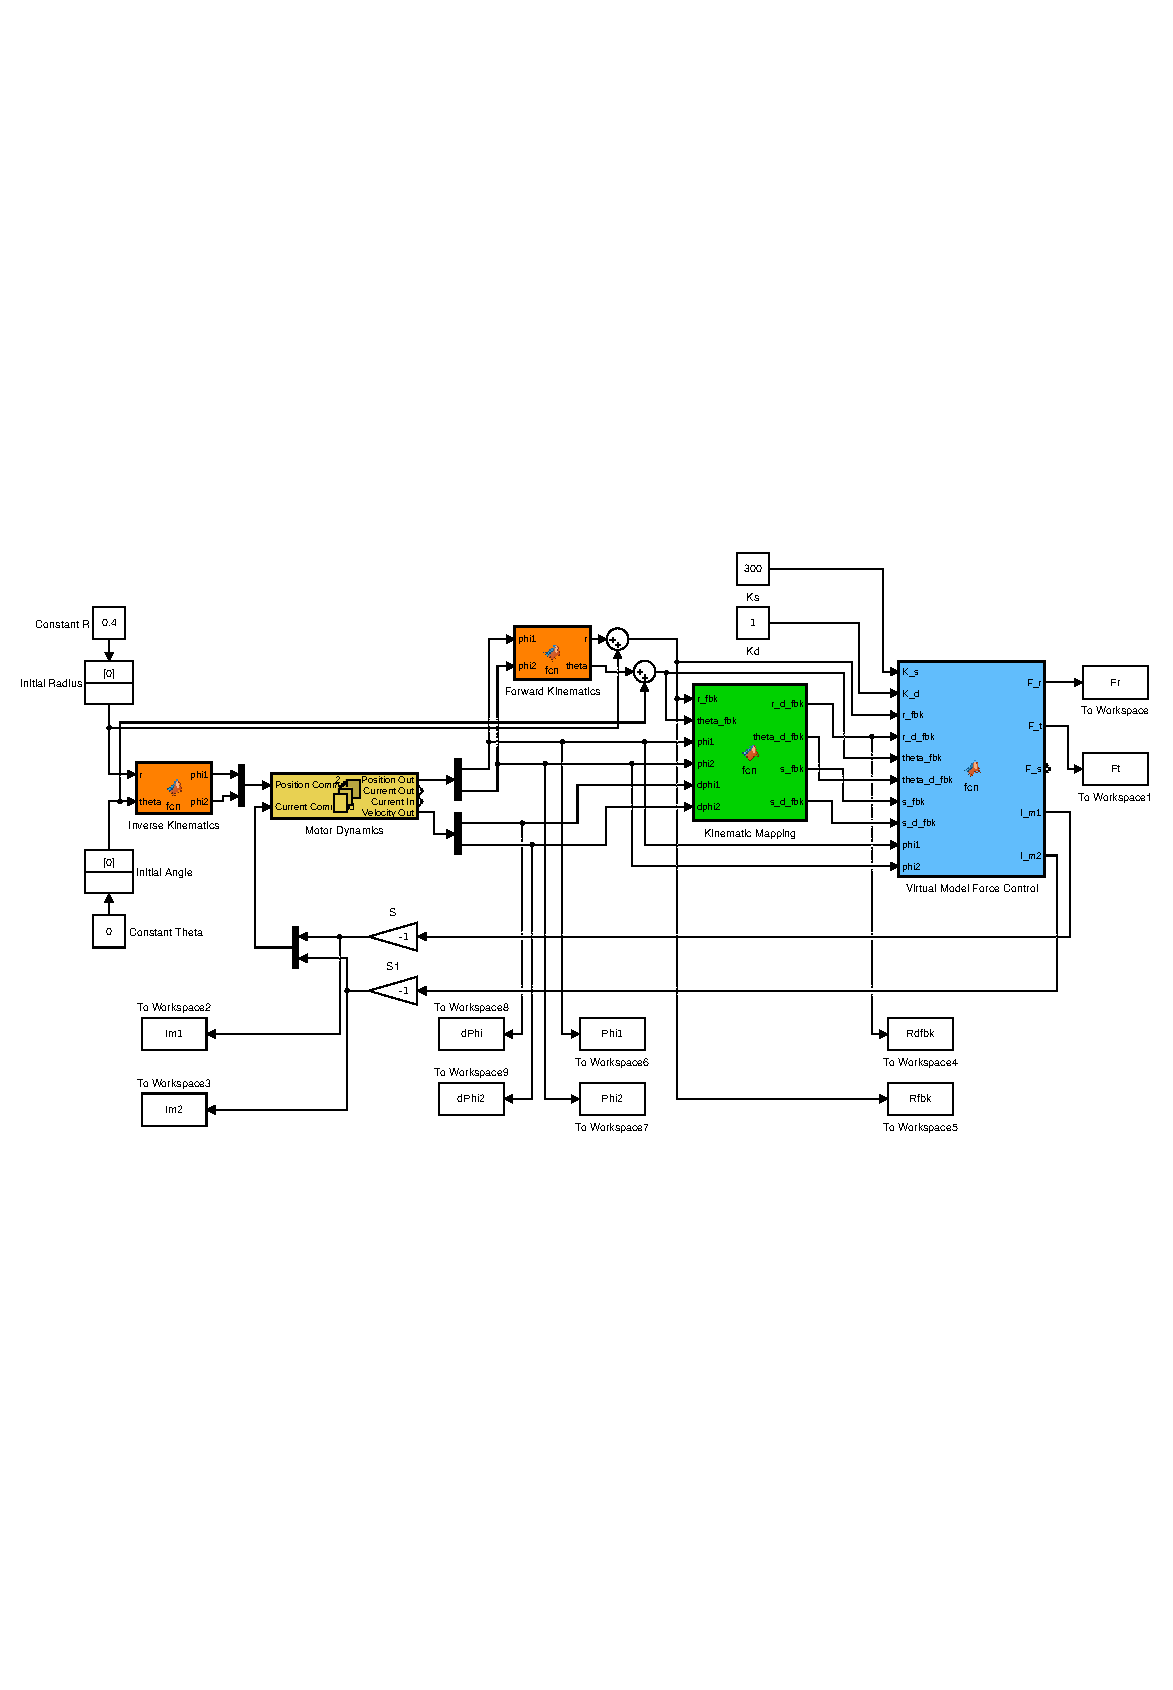
\includegraphics[width=1\textwidth]{images/simulation/leg-simulation.eps}
\caption{a}
\label{fig:a}
\end{figure}

\begin{figure}
\centering
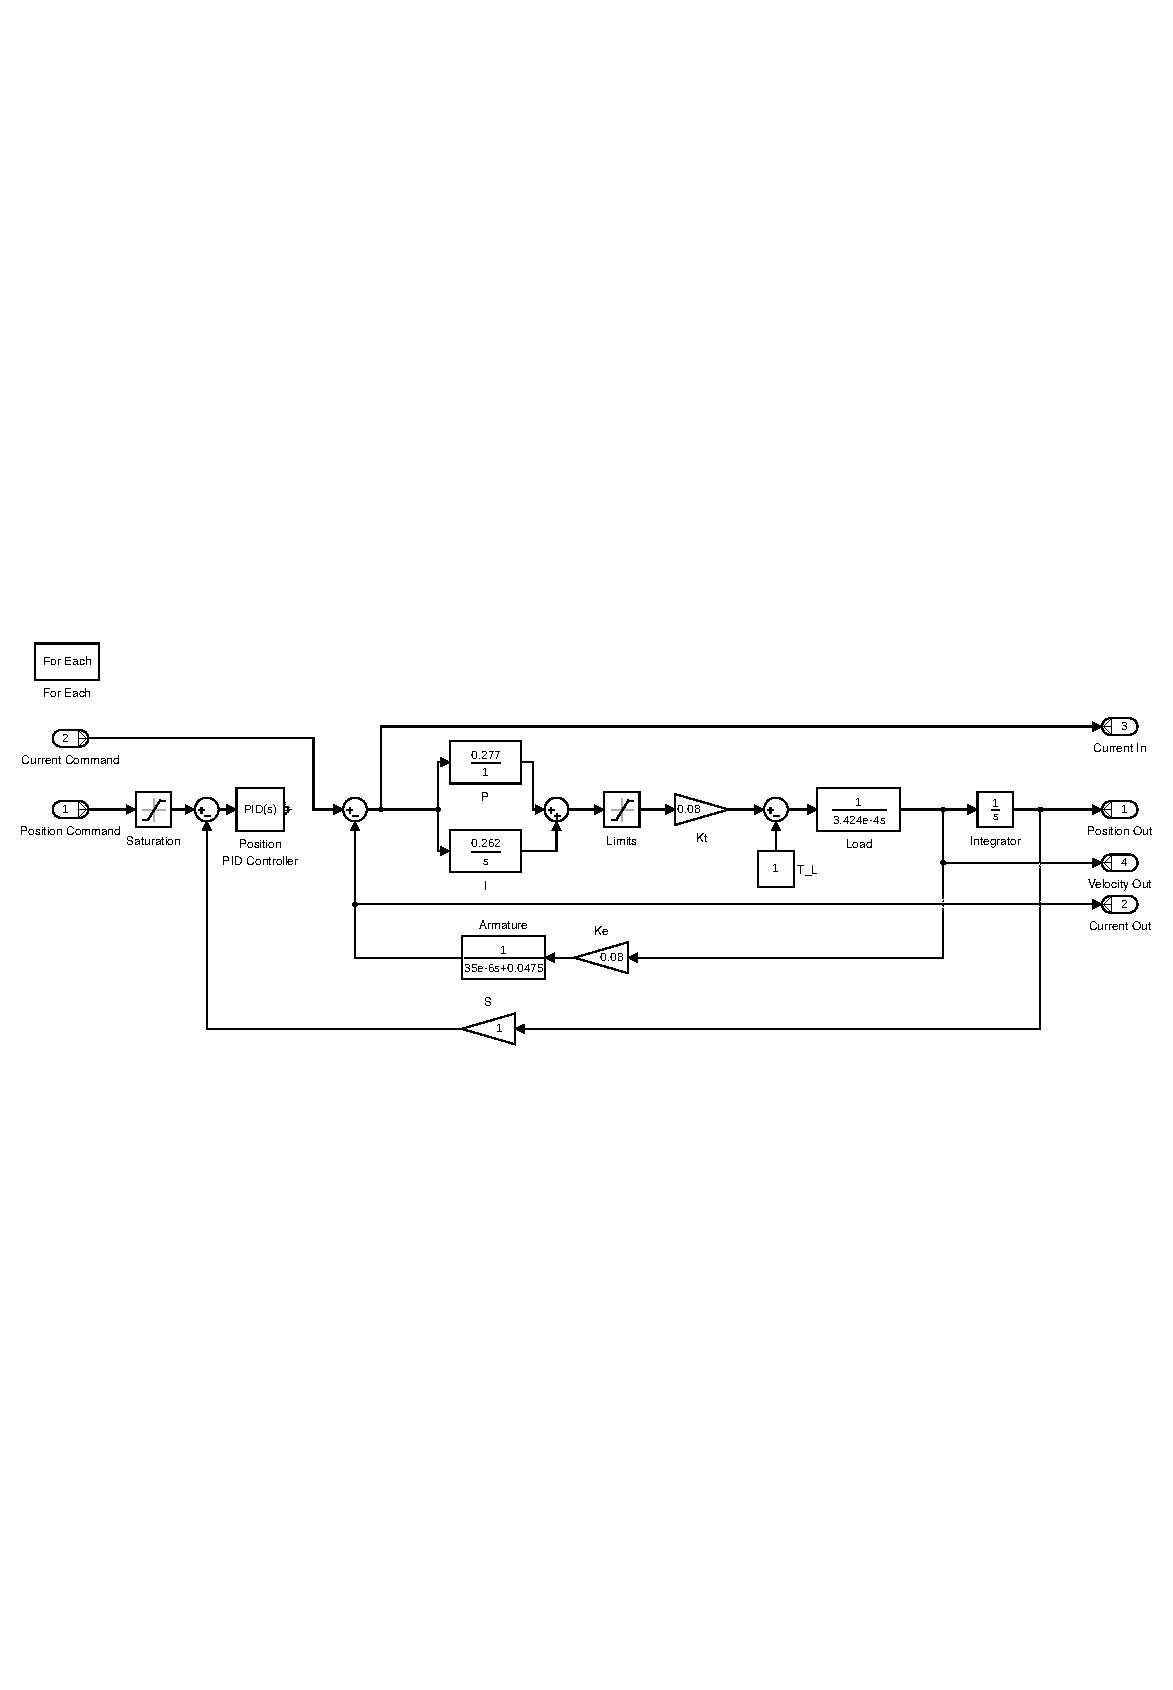
\includegraphics[width=1\textwidth]{images/simulation/motor-model.eps}
\caption{a}
\label{fig:a}
\end{figure}

\begin{figure}
\centering
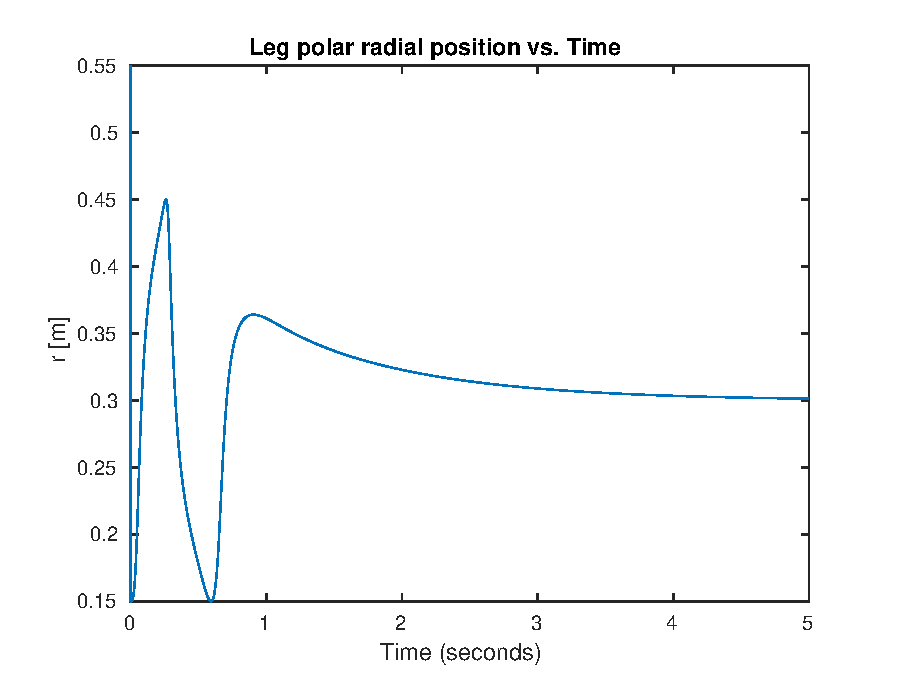
\includegraphics[width=1\textwidth]{images/simulation/r.eps}
\caption{a}
\label{fig:a}
\end{figure}

\begin{figure}
\centering
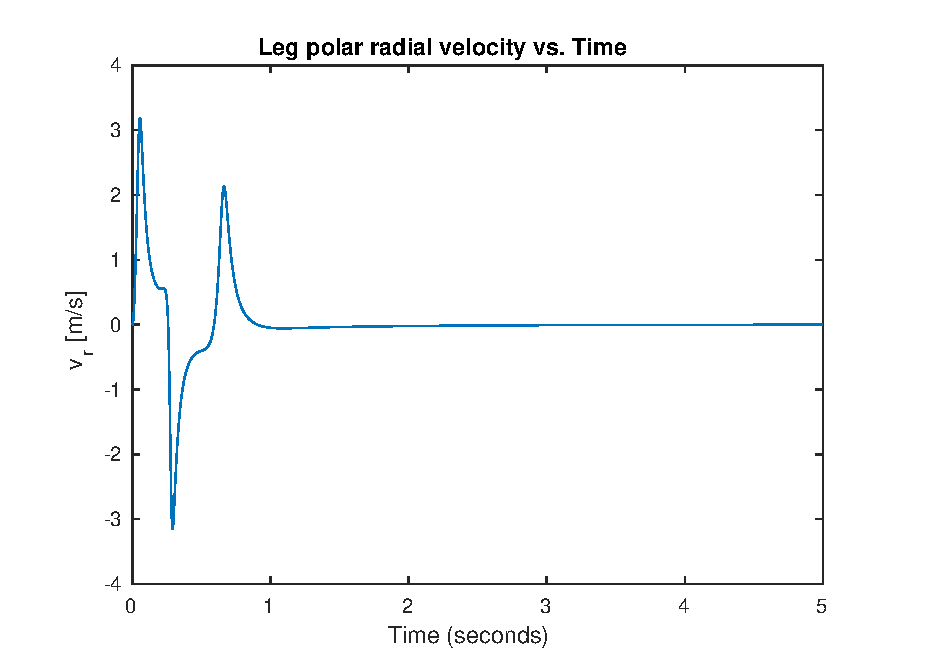
\includegraphics[width=1\textwidth]{images/simulation/vr.eps}
\caption{a}
\label{fig:a}
\end{figure}

\begin{figure}
\centering
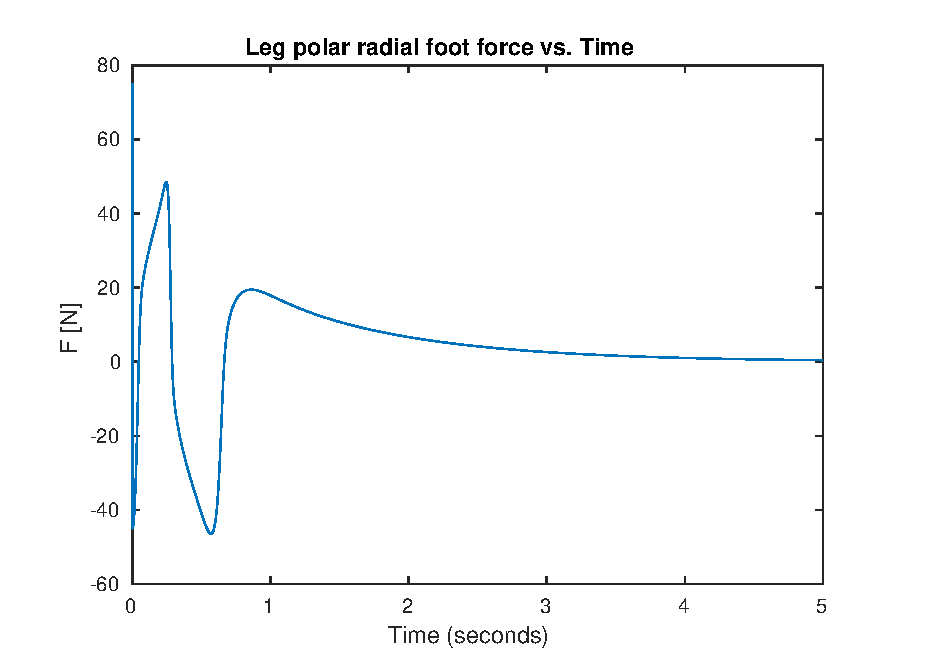
\includegraphics[width=1\textwidth]{images/simulation/f.eps}
\caption{a}
\label{fig:a}
\end{figure}

\begin{figure}
\centering
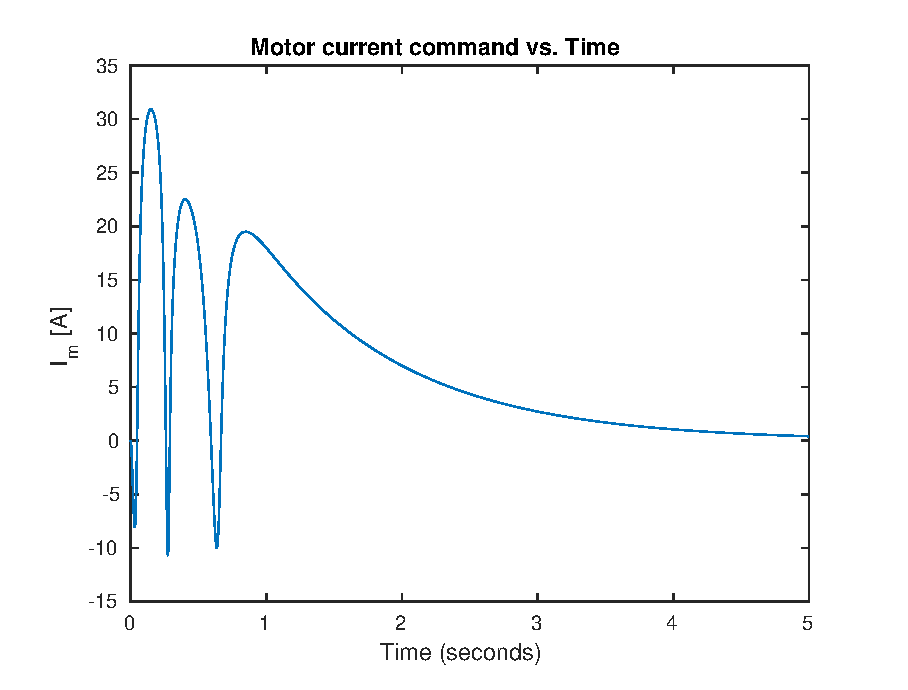
\includegraphics[width=1\textwidth]{images/simulation/im.eps}
\caption{a}
\label{fig:a}
\end{figure}